\documentclass{article}
\usepackage{amsmath, amsthm, amssymb}
\usepackage{tikz}
\usepackage{array}
\usepackage{graphicx} % Added for including the PDF file as an image
\usepackage{float}
\usepackage{mathpazo}
\usetikzlibrary{angles, quotes}
\usepackage{longdivision}
\usepackage[margin=1in]{geometry}
\begin{document}
\section*{\huge Mathematics Homework Sheet 3}
\begin{flushright}
   \textbf{Authors: Abdullah Oguz Topcuoglu \& Ahmed Waleed Ahmed Badawy Shora}
\end{flushright}

% 1. Find all complex solutions of the following equations.
% (a) 3z
% 2 + z = 1
% (b) 3z
% 2 + z = 0
% (c) z
% 2 − (3 + i)z + 4 + 3i = 0
% (d) sinh z = i
% (e) tan z = 1
% (f) cos z = −
% 5
% 4
% (g) z + ¯z = 1
% (h) z
% 2 + 2¯z
% 2 + z − z¯ + 9 = 0
% (i) (1 − i)z
% 2 = 1 + 7i
% (j) (1 − i)z
% 2 = (1 + i)z
% (k) z
% 4 − 4z
% 2 + 16 = 0
% (l) z
% 3 = 1
% (m) (z
% 2 − 1)3 = 8z
% 3
% (n) z
% 4 + 1 = 0
% (o) z
% 6 − 3iz
% 3 − 2 = 0
% (p) z
% 3 + 2z
% 2 + 2z = 0
% (q) e
% z = 1
% (r) e
% z = eiz
% (s) e
% iz + 4e−iz = 4
% (t) e
% 2z + iez + 1 = 0
% 2. Let
% A = {z ∈ C : |z − 2 − 3i| < |z + 4 − 5i|},
% B = {z ∈ C : 0 ≤ arg(z + 3 − 4i) < π/4}.
% Sketch the sets A, B and A ∩ B.
% 3. a) Compute (4√
% 3 − 4i)88
% .
% b) Let m and n be natural numbers and
% z =
% 
% 1 + i tan 
% (4m + 1)π
% 4n
% n
% .
% Find Re z und Im z.
% [Hint: Use de Moivre’s theorem.]
% 4. Prove that (C, +, ·) is not an ordered field. [Hint: Show that each of the assumptions
% i > 0 and i < 0 lead to a contradiction.]

\section*{Problem 1}

% 1. Find all complex solutions of the following equations.
% (a) 3z
% 2 + z = 1
% (b) 3z
% 2 + z = 0
% (c) z
% 2 − (3 + i)z + 4 + 3i = 0
% (d) sinh z = i
% (e) tan z = 1
% (f) cos z = −
% 5
% 4
% (g) z + ¯z = 1
% (h) z
% 2 + 2¯z
% 2 + z − z¯ + 9 = 0
% (i) (1 − i)z
% 2 = 1 + 7i
% (j) (1 − i)z
% 2 = (1 + i)z
% (k) z
% 4 − 4z
% 2 + 16 = 0
% (l) z
% 3 = 1
% (m) (z
% 2 − 1)3 = 8z
% 3
% (n) z
% 4 + 1 = 0
% (o) z
% 6 − 3iz
% 3 − 2 = 0
% (p) z
% 3 + 2z
% 2 + 2z = 0
% (q) e
% z = 1
% (r) e
% z = eiz
% (s) e
% iz + 4e−iz = 4
% (t) e
% 2z + iez + 1 = 0

\subsection*{(a)}
\[
   3z^2 + z = 1
\]

solve the quadratic equations and we get
\[
   z = \frac{-1 \pm \sqrt{1^2 - 4.3.(-1)}}{(3.2)}
\]
\[
   z = \frac{-1 \pm \sqrt{1 + 12}}{6}
\]
\[
   z = \frac{-1 \pm \sqrt{13}}{6}
\]
\[
   z_0 = \frac{-1 + \sqrt{13}}{6} + 0i, \quad z_1 = \frac{-1 - \sqrt{13}}{6} + 0i
\]

\subsection*{(b)}
\[
   3z^2 + z = 0
\]
\[
   z(3z + 1) = 0
\]
\[
   z = 0 \quad \text{or} \quad 3z + 1 = 0
\]
\[
   z = 0 \quad \text{or} \quad z = -\frac{1}{3}
\]

\subsection*{(c)}
\[
   z^2 - (3 + i)z + 4 + 3i = 0
\]
\[
   z = \frac{(3 + i) \pm \sqrt{(3 + i)^2 - 4(4 + 3i)}}{2}
\]
\[
   z = \frac{(3 + i) \pm \sqrt{(9 + 6i - 1 - 16 - 12i)}}{2}
\]
\[
   z = \frac{(3 + i) \pm \sqrt{-8 - 6i}}{2}
\]
\[
   z = \frac{(3 + i) \pm (1 - 3i)}{2}
\]
\[
   z_0 = \frac{4 - 2i}{2} = 2 - i, \quad z_1 = \frac{2 + 4i}{2} = 1 + 2i
\]

\(\sqrt{-8 - 6i} = \pm (1 - 3i)\) because \(\sqrt{-8 - 6i} = \pm (\sqrt{\frac{r+(-8)}{2}} + sign(-6)\sqrt{\frac{r-(-8)}{2}}i)\) where \(r = |-8 -6i|\)

\subsection*{(d)}

\[
   \sinh z = i
\]
By definiton of sinh
\[
   \frac{e^z - e^{-z}}{2} = i
\]
Multiplying both sides by \(2e^z\), we get:
\[e^{2z} - 1 = 2ie^z\]
\[e^{2z} - 2ie^z -1 = 0\]
Solving for \(e^z\) with \(a= 1, b = -2i, c = -1
\):
\[e^z = \frac{2i}{2}\pm \sqrt{\frac{-4+4}{4}} = i=1\cdot e^{i\frac{\pi}{2}}\]
\[z= i(\frac{\pi}{2}+2n\pi), n\in\mathbb{Z}\]

\subsection*{(e)}
\[
   tan(z) = 1
\]
\[
   \frac{sin(z)}{cos(z)} = 1
\]
\[
   sin(z) = cos(z)
\]
By definition of sin(z) and cos(z)
\[
   \frac{e^{iz} - e^{-iz}}{2i} = \frac{e^{iz} + e^{-iz}}{2}
\]
\[
   e^{iz} - e^{-iz} = i(e^{iz} + e^{-iz})
\]
   \[e^{2iz} - 1 = i(e^{2iz} + 1)\]
   \[e^{2iz}(1-i) = 1+i\]
   \[e^{2iz}= \frac{1+i}{1-i} = \frac{\sqrt{2}e^{i\frac{\pi}{4}}}{\sqrt{2}e^{-i\frac{\pi}{4}}} = e^{i\frac{\pi}{2}}\]
   \[2z=\frac{\pi}{2} + 2n\pi , n \in \mathbb{Z}\]
   \[z=\frac{\pi}{4} + n\pi , n \in \mathbb{Z}\]

\subsection*{(f)}
\[
   cos(z) = -\frac{5}{4}
\]
By definition of cos(z)
\[
   \frac{e^{iz} + e^{-iz}}{2} = -\frac{5}{4}
\]
\[
   e^{iz} + e^{-iz} = -\frac{5}{2}
\]
Let \(q = e^{iz}\)
\[
   q + \frac{1}{q} = -\frac{5}{2}
\]
\[
   q^2 + \frac{5}{2}q + 1 = 0
\]
\[
   q = \frac{-\frac{5}{2} \pm \sqrt{(\frac{5}{2})^2 - 4}}{2}
\]
\[
   q = \frac{-\frac{5}{2} \pm \frac{3}{2}}{2}
\]
\[
   q_0 = \frac{-1}{2}, \qquad q_1 = -2
\]
\[
   e^{iz_0} = -\frac{1}{2} = \frac{1}{2}e^{i\pi}
\]
\[
   e^{iz_0 -i\pi} = \frac{1}{2}
\]
\[
   iz_0 - i\pi = ln(\frac{1}{2})
\]
\[
   z_0 = \frac{ln(\frac{1}{2}) + i\pi}{i}
\]

\[
   e^{iz_1} = -2 = 2e^{i\pi}
\]
\[
   e^{iz_1 - i\pi} = 2
\]
\[
   iz_1 - i\pi = ln(2)
\]
\[
   z_1 = \frac{ln(2) + i\pi}{i}
\]

\subsection*{(g)}
\[
   z + \bar{z} = 1
\]
Let \(z = x + iy\)
\[
   x + iy + x - iy = 1
\]
\[
   2x = 1
\]
\[
   x = \frac{1}{2}
\]
\[
   z = \frac{1}{2} + iy, \qquad y \in R
\]

\subsection*{(h)}
\[
   z^2 + 2\bar{z}^2 + z - \bar{z} + 9 = 0
\]
Let \(z = x + iy\)
\[
   (x + iy)^2 + 2(x - iy)^2 + (x + iy) - (x - iy) + 9 = 0
\]
\[
   9 - 2iy + x^2 + 2xyi - y^2 + 2x^2 - 4xyi -2y^2 = 0
\]
\[
   9 - 2iy + 3x^2 - 2xyi - 3y^2 = 0
\]
\[
   9 + 3x^2 - 3y^2 = 0, \quad -2y - 2xy = 0
\]
\[
   x = 1
\]
Insert this in the first equation
\[
   9 + 3 - 3y^2 = 0
\]
\[
   y^2 = 4
\]
\[
   y =  \pm 2
\]

\[
   z = 1\pm2i 
\]
\subsection*{(i)}
\[(1 - i)z^2 = 1 + 7i\]
\[z^2 = \frac{1 + 7i}{1-i} = \frac{(1+7i)(1+i)}{2} = \frac{1+i+7i-7}{2} = -3+4i \]
\[z = \pm \sqrt{-3+4i}\]
\subsection*{(j)}
\[(1 - i)z^2 = (1 + i)z\]
\[
(1 - i)z^2 - (1 + i)z = 0
\]
\[
z\left[(1 - i)z - (1 + i)\right] = 0
\]
\[
z = 0 \quad \text{or} \quad (1 - i)z = 1 + i
\]

\[
z = \frac{1 + i}{1 - i} = \frac{(1 + i)(1 + i)}{(1 - i)(1 + i)} = \frac{(1 + 2i + i^2)}{1 + 1} = \frac{1 + 2i -1}{2} = \frac{2i}{2} = i
\]

\[
\Rightarrow z = 0 \quad \text{or} \quad z = i
\]
\subsection*{(k)}
\[z^4-4z^2+16=0\]
Solving for $z^2$ using a = 1, b = -4 and c = 16, we get:
\[z^2 =\frac{4\pm\sqrt{16-4\cdot16}}{2} = 2\pm\frac{\sqrt{-48}}{2} = 2\pm 2\sqrt{3} i  = 4e^{\pm i\frac{\pi}{3}}\]
\[z=\pm 2e^{\pm i\frac{\pi}{6}}\]
\subsection*{(l)}
\[z^3 = 1 \]
We know that $z=1$ is one of the solutions.
We divide \( z^3 - 1 \) by \( z - 1 \) using polynomial long division:


\begin{align*}
&\underline{z^3 - 1 \div z - 1} \\
&\text{Step 1: } z^3 \div z = z^2 \\
&\quad \Rightarrow z^2(z - 1) = z^3 - z^2 \\
&\quad \text{Subtract: } (z^3 - 1) - (z^3 - z^2) = z^2 - 1 \\
\\
&\text{Step 2: } z^2 \div z = z \\
&\quad \Rightarrow z(z - 1) = z^2 - z \\
&\quad \text{Subtract: } (z^2 - 1) - (z^2 - z) = z - 1 \\
\\
&\text{Step 3: } z \div z = 1 \\
&\quad \Rightarrow 1(z - 1) = z - 1 \\
&\quad \text{Subtract: } (z - 1) - (z - 1) = 0 \\
\\
&\therefore \quad \frac{z^3 - 1}{z - 1} = z^2 + z + 1
\end{align*}
\[z^3-1=(z-1)(z^2 + z + 1) = 0\]
\[z= -\frac{1}{2}\pm\sqrt{-\frac{3}{4}} = -\frac{1}{2}\pm\frac{\sqrt{3}}{2}i \]
\[z = 1 \quad\text{or} \quad z= -\frac{1}{2}\pm\frac{\sqrt{3}}{2}i\]
\subsection*{(m)}
\[
(z^2 - 1)^3 = (2z)^3
\;\Longrightarrow\;
z^2 - 1 = 2z,\quad
z^2 - 1 = 2z\Bigl(-\tfrac12 + i\tfrac{\sqrt3}{2}\Bigr),\quad
z^2 - 1 = 2z\Bigl(-\tfrac12 - i\tfrac{\sqrt3}{2}\Bigr).
\]

% Case 1: root = 1
\textbf{Case 1:}\quad $z^2 - 1 = 2z$
\[
z^2 - 2z - 1 = 0
\quad\Longrightarrow\quad
z = \frac{2 \pm \sqrt{8}}{2} = 1 \pm \sqrt2.
\]

% Case 2: root = -1/2 + i√3/2
\textbf{Case 2:}\quad $z^2 - 1 = 2z\bigl(-\tfrac12 + i\tfrac{\sqrt3}{2}\bigr)$
\[
z^2 + \bigl(1 - i\sqrt3\bigr)z - 1 = 0
\quad\Longrightarrow\quad
z = \frac{-\,(1 - i\sqrt3) \pm \sqrt{(1 - i\sqrt3)^2 + 4}}{2}
= \frac{-1 + \sqrt3}{2} \pm i\,\frac{\sqrt3 - 1}{2}.
\]

% Case 3: root = -1/2 - i√3/2
\textbf{Case 3:}\quad $z^2 - 1 = 2z\bigl(-\tfrac12 - i\tfrac{\sqrt3}{2}\bigr)$
\[
z^2 + \bigl(1 + i\sqrt3\bigr)z - 1 = 0
\quad\Longrightarrow\quad
z = \frac{-\,(1 + i\sqrt3) \pm \sqrt{(1 + i\sqrt3)^2 + 4}}{2}
= \frac{-1 - \sqrt3}{2} \pm i\,\frac{\sqrt3 + 1}{2}.
\]

\bigskip

\[
\boxed{
\begin{aligned}
&z = 1 \pm \sqrt2,\\
&z = \frac{-1 + \sqrt3}{2}\,\pm\,i\,\frac{\sqrt3 - 1}{2},\\
&z = \frac{-1 - \sqrt3}{2}\,\pm\,i\,\frac{\sqrt3 + 1}{2}.
\end{aligned}
}
\]
\subsection*{(n)}
\[
z^4 + 1 = 0
\;\Longrightarrow\;
z^4 = -1 = e^{i(\pi + 2\pi k)},\quad k\in \mathbb{Z}
\]
\[
z = e^{i\bigl(\frac{\pi + 2\pi k}{4}\bigr)}
    = e^{i\bigl(\tfrac\pi4 + \tfrac{\pi k}{2}\bigr)},
\quad k\in \mathbb{Z}
\]
Taking k s that will get us an angle in  $(-\pi,\pi]$,
\[
z = e^{i\pi/4},\; e^{i3\pi/4},\; e^{i5\pi/4},\; e^{i7\pi/4},
\]
\subsection*{(o)}
\[
z^6 - 3i\,z^3 - 2 = 0.
\]
Set \(w = z^3\).  Then
\[
w^2 - 3i\,w - 2 = 0
\;\Longrightarrow\;
w = \frac{3i \pm \sqrt{(-3i)^2 + 8}}{2}
= \frac{3i \pm i}{2}
= \begin{cases}2i,\\[4pt]i.\end{cases}
\]
Hence we must solve
\[
z^3 = 2i
\quad\text{and}\quad
z^3 = i.
\]
By taking cube-roots (as in your solution of \(z^3=1\)), we get

1. For \(z^3=2i=2e^{i\pi/2}\):
\[
z = (2)^{1/3} \exp\!\Bigl(i\frac{\pi/2 + 2\pi k}{3}\Bigr)
= 2^{1/3}e^{\,i(\pi/6 + 2\pi k/3)},\quad k=0,1,2.
\]

2. For \(z^3=i=e^{i\pi/2}\):
\[
z = \exp\!\Bigl(i\frac{\pi/2 + 2\pi k}{3}\Bigr)
= e^{\,i(\pi/6 + 2\pi k/3)},\quad k=0,1,2.
\]

Thus the six solutions are
\[
\boxed{
z = 2^{1/3}e^{\,i(\pi/6 + 2\pi k/3)},\quad
z = e^{\,i(\pi/6 + 2\pi k/3)},
\quad k=0,1,2.
}
\]
\subsection*{(p)}
We factor first:
\[
z^3 + 2z^2 + 2z = z(z^2 + 2z + 2) = 0.
\]

One solution is:
\[
z = 0.
\]

For the quadratic \(z^2 + 2z + 2 = 0\), use the quadratic formula with \(a = 1\), \(b = 2\), \(c = 2\):
\[
z = \frac{-2 \pm \sqrt{2^2 - 4 \cdot 1 \cdot 2}}{2 \cdot 1}
= \frac{-2 \pm \sqrt{-4}}{2}
= \frac{-2 \pm 2i}{2}
= -1 \pm i.
\]

\[
\boxed{z = 0,\quad z = -1 + i,\quad z = -1 - i}
\]
\subsection*{(q)}
We write \(1 = e^{2\pi i k}\), so:
\[
e^z = e^{2\pi i k} \Rightarrow z = 2\pi i k, \quad k \in \mathbb{Z}.
\]
\[
\boxed{z = 2\pi i k}
\]
\subsection*{(r)}
We solve:
\[
e^z = e^{iz}.
\]

Equating exponents up to a multiple of \(2\pi i\), we write:
\[
z = iz + 2\pi i k, \quad k \in \mathbb{Z}.
\]

Solving:
\[
z - iz = 2\pi i k
\Rightarrow z(1 - i) = 2\pi i k
\Rightarrow z = \frac{2\pi i k}{1 - i}.
\]

Multiply numerator and denominator by \(1 + i\):
\[
z = \frac{2\pi i k (1 + i)}{2} = \pi i k (1 + i).
\]

Now write:
\[
z = \pi k i (1 + i) = \pi k (-1 + i), \quad \text{since } i^2 = -1.
\]

So:
\[
\boxed{z = \pi k(-1 + i), \quad k \in \mathbb{Z}}
\]

\textbf{Restricting to angles in } \((- \pi, \pi]\), we consider only values of \(k\) such that:
\[
\arg(e^z) = \arg(e^{iz}) \in (-\pi, \pi]
\Rightarrow \text{we need } \operatorname{Im}(z) = \pi k \in (-\pi, \pi].
\]

Thus \(k = -1, 0, 1\). Therefore:
\[
\boxed{
\begin{aligned}
k = -1 &\Rightarrow z = \pi (1 - i) \\
k = 0 &\Rightarrow z = 0 \\
k = 1 &\Rightarrow z = \pi (-1 + i)
\end{aligned}
}
\]

Final boxed form:
\[
\boxed{
z \in \left\{ \pi(1 - i),\; 0,\; \pi(-1 + i) \right\}
}
\]
\subsection*{(s)}
Given:
\[
e^{iz} + 4e^{-iz} = 4
\]

Multiply both sides by \(e^{iz}\):
\[
e^{2iz} + 4 = 4e^{iz}
\Rightarrow e^{2iz} - 4e^{iz} + 4 = 0
\]

Let \(w = e^{iz}\), then:
\[
w^2 - 4w + 4 = 0
\Rightarrow (w - 2)^2 = 0 \Rightarrow w = 2
\]

Now solve:
\[
e^{iz} = 2 \Rightarrow iz = \ln 2 + 2\pi i k
\Rightarrow z = -i \ln 2 + 2\pi k, \quad k \in \mathbb{Z}
\]

\[
\boxed{z = 2\pi k - i \ln 2}
\]
\subsection*{(t)}
Given:
\[
e^{2z} + i e^z + 1 = 0
\]

Let \(w = e^z\), then:
\[
w^2 + i w + 1 = 0
\Rightarrow w = \frac{-i \pm \sqrt{i^2 - 4}}{2} = \frac{-i \pm \sqrt{-1 - 4}}{2} = \frac{-i \pm \sqrt{-5}}{2}
\]

\[
w = \frac{-i \pm i\sqrt{5}}{2} = i \cdot \frac{-1 \pm \sqrt{5}}{2}
\]

Now solve \(e^z = w\):
\[
z = \ln\left(i \cdot \frac{-1 \pm \sqrt{5}}{2}\right) + 2\pi i k
\]

\[
\boxed{z = \ln\left(i \cdot \tfrac{-1 \pm \sqrt{5}}{2}\right) + 2\pi i k}
\]
\section*{Problem 2}
%--------------------
\section*{Set \(A\)}
\[
A = \{z\in\mathbb{C} : |z-(2+3i)| < |z-(-4+5i)|\},
\]
i.e.\ the half‐plane on the side of the perpendicular bisector of \((2,3)\)--\((-4,5)\)\,containing \((2,3)\).
\begin{center}
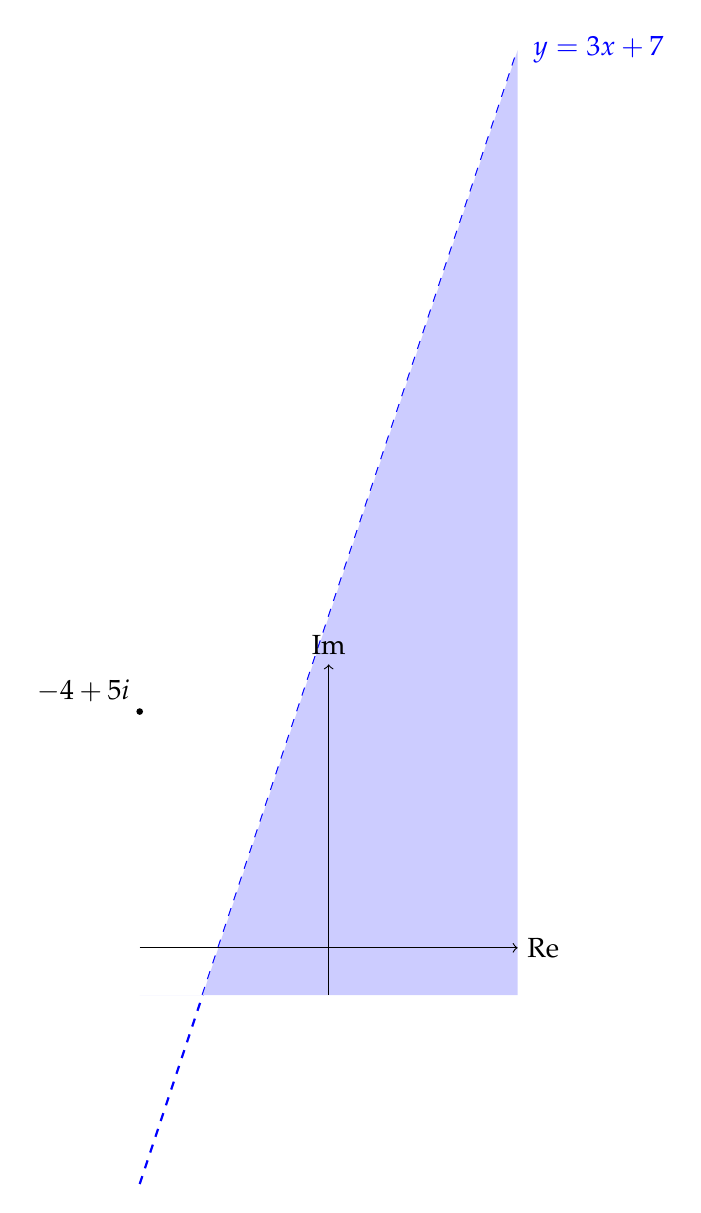
\begin{tikzpicture}[scale=0.6]
  % Points
  \coordinate (P) at (2,3);
  \coordinate (Q) at (-4,5);
  \fill (P) circle (2pt) node[below right] {\(2+3i\)};
  \fill (Q) circle (2pt) node[above left]  {\(-4+5i\)};

  % Perpendicular bisector: y = 3x + 7
  \draw[thick,dashed,blue] plot[domain=-4:4] (\x,{3*\x+7})
    node[right, xshift=2pt] {\(y=3x+7\)};

  % Shade region closer to P (below the bisector)
  % Intersection of bisector and bottom y=-1: x = -8/3 ≈ -2.6667
  \fill[blue!20]
    (-4,-1) -- (4,-1) -- (4,{3*4+7})
    -- plot[domain=4:-2.6667] (\x,{3*\x+7}) -- cycle;

  % Axes
  \draw[->] (-4,0)--(4,0) node[right]{Re};
  \draw[->] (0,-1)--(0,6) node[above]{Im};
\end{tikzpicture}
\end{center}

%--------------------
\section*{Set \(B\)}
\[
B = \{z\in\mathbb{C} : 0 \le \arg(z + 3 - 4i) < \tfrac\pi4\},
\]
i.e.\ the sector with vertex \(-3+4i\), between ray at angle \(0\) and \(\pi/4\).
\begin{center}
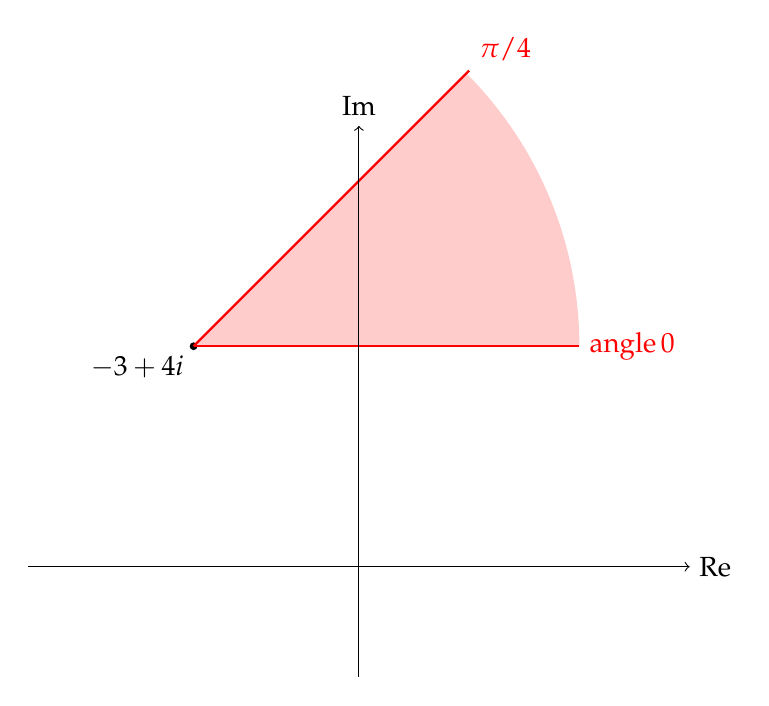
\begin{tikzpicture}[scale=0.7]
  % Vertex
  \coordinate (V) at (-3,4);
  \fill (V) circle (2pt) node[below left]{\(-3+4i\)};
  % Sector fill
  \fill[red!20]
    (V) -- ++(7,0)
    arc[start angle=0,end angle=45,radius=7cm]
    -- cycle;
  % Boundary rays
  \draw[thick,red] (V)--++(7,0) node[right]{angle\,0};
  \draw[thick,red] (V)--++(5,5) node[above right]{\(\pi/4\)};
  % Axes
  \draw[->] (-6,0)--(6,0) node[right]{Re};
  \draw[->] (0,-2)--(0,8) node[above]{Im};
\end{tikzpicture}
\end{center}

%--------------------
\section*{Intersection \(A\cap B\)}
Shade only the points satisfying both conditions.
\begin{center}
\begin{tikzpicture}[scale=0.6]
  % Key points
  \coordinate (P) at (2,3);
  \coordinate (Q) at (-4,5);
  \coordinate (V) at (-3,4);

  % Axes
  \draw[->] (-6,0) -- (6,0) node[right]{Re};
  \draw[->] (0,-2) -- (0,8) node[above]{Im};

  % Perp-bisector of PQ: y=3x+7
  \draw[dashed, blue, thick]
    plot[domain=-6:6] (\x, {3*\x + 7});

  % Sector rays from V
  \draw[red, thick] (V) -- ++(7,0) node[right]{0};
  \draw[red, thick] (V) -- ++(5,5) node[above right]{$\tfrac\pi4$};

  % Intersection fill
  \begin{scope}
    % clip to A: half-plane below y=3x+7
    \clip 
      (-10,-10) -- (10,-10) --
      plot[domain=10:-10] (\x, {3*\x + 7}) -- cycle;
    % clip to B: sector at V
    \clip 
      (V) -- ++(7,0)
      arc[start angle=0,end angle=45,radius=7cm] -- cycle;
    % fill overlap
    \fill[purple!50] (-10,-10) rectangle (10,10);
  \end{scope}
\end{tikzpicture}
\end{center}
\section*{Problem 3}
\subsection*{(a)}
\[
   (4\sqrt{3} - 4i)^{88}
\]
Let's convert this to polar form
\[
   r = \sqrt{(4\sqrt{3})^2 + (-4)^2} = \sqrt{48 + 16} = \sqrt{64} = 8
\]
\[
   \theta = tan^{-1}(\frac{-4}{4\sqrt{3}}) = tan^{-1}(-\frac{1}{\sqrt{3}}) = -\frac{\pi}{6}
\]
So we want to compute
\[
   (8e^{-\frac{\pi}{6}i})^{88}
\]
\[
   (8e^{-\frac{\pi}{6}i})^{88} = 8^{88}e^{-\frac{88\pi}{6}i} = 8^{88}e^{-\frac{44\pi}{3}i}
\]

\subsection*{(b)}

\[
   z = \left(1 + i \tan\left(\frac{(4m + 1)\pi}{4n}\right)\right)^n
\]
\[
   z = \left(1 + i \frac{\sin\left(\frac{(4m + 1)\pi}{4n}\right)}{\cos\left(\frac{(4m + 1)\pi}{4n}\right)}\right)^n
\]
\[
   z = \left(\frac{ \cos\left(\frac{(4m + 1)\pi}{4n}\right)  + i\sin\left(\frac{(4m + 1)\pi}{4n}\right)  }{\cos\left(\frac{(4m + 1)\pi}{4n}\right)}\right)^n
\]
\[
   z = \left(\frac{1}{\cos\left(\frac{(4m + 1)\pi}{4n}\right)}\right)^n \left(\cos\left(\frac{(4m + 1)\pi}{4n}\right) + i\sin\left(\frac{(4m + 1)\pi}{4n}\right)\right)^n
\]
Using de Moivre's theorem
\[
   z = \frac{1}{\cos\left(\frac{(4m + 1)\pi}{4n}\right)^n} \left(\cos\left(\frac{(4m + 1)\pi}{4}\right) + i\sin\left(\frac{(4m + 1)\pi}{4}\right)\right)
\]
\[
   Re(z) = \frac{1}{\cos\left(\frac{(4m + 1)\pi}{4n}\right)^n} \cos\left(\frac{(4m + 1)\pi}{4}\right)
\]
\[
   Im(z) = \frac{1}{\cos\left(\frac{(4m + 1)\pi}{4n}\right)^n} \sin\left(\frac{(4m + 1)\pi}{4}\right)
\]

\section*{Problem 4}

% 4. Prove that (C, +, ·) is not an ordered field. [Hint: Show that each of the assumptions
% i > 0 and i < 0 lead to a contradiction.]
In an ordered field the following must hold \(0 < 1\) \\
Assume \(i > 0\)

\begin{align*}
   0 &< i & \text{(multiply by i)}\\
   0 &< i^2 & \text{}\\
   0 &< -1 & \text{(add 1)}\\
   1 &< 0 & \text{this is a contradiction}\\
\end{align*}
\\
Assume \(i < 0\)
\begin{align*}
   0 &< -i & \text{(multiply by -i)}\\
   0 &< i^2 & \text{}\\
   0 &< -1 & \text{(add 1)}\\
   1 &< 0 & \text{this is a contradiction}\\
\end{align*}

Thus, we have shown that both assumptions lead to a contradiction. Therefore, \((C, +, \cdot)\) is not an ordered field.

\end{document}